\chapter{RESULTS}

\section{User \& Account Creation}

\begin{figure}[h!]
    \centering
    
\includegraphics[width=0.5\textwidth]{Graphics/agile.png}
    \caption{Agile Model}
\end{figure}

Spandan xito user and account creation css milau.



\section{Posting Status With Latex}

Users can write mathematical expressions using LaTeX syntax while composing a post. As shown in Figure 5.2, the application provides a live preview of the rendered LaTeX output, allowing users to verify their equations before posting. Once published, the post is displayed in the timeline with properly formatted LaTeX expressions, as demonstrated in Figure 5.3. This feature ensures that complex mathematical notations, scientific formulas, and equations are easily readable and visually appealing in posts.

\begin{figure}[htbp]
  \centering
  % First image in its own minipage
  \begin{minipage}[b]{0.45\linewidth}
    \centering
    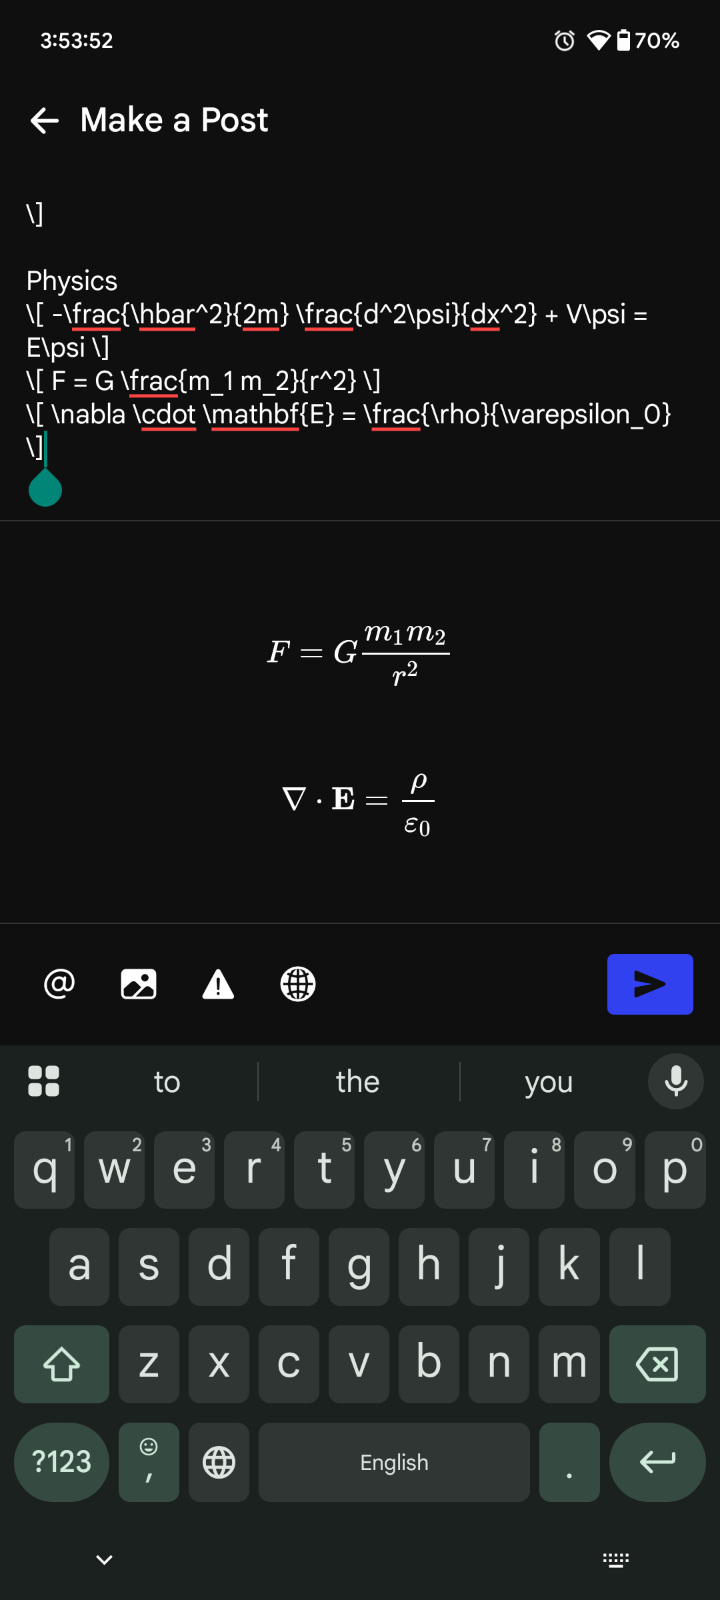
\includegraphics[width=\linewidth]{Graphics/writingpost.png}
    \caption{Live rendering of latex while writing post}
  \end{minipage}
  \hfill % adds some space between images
  % Second image in its own minipage
  \begin{minipage}[b]{0.45\linewidth}
    \centering
    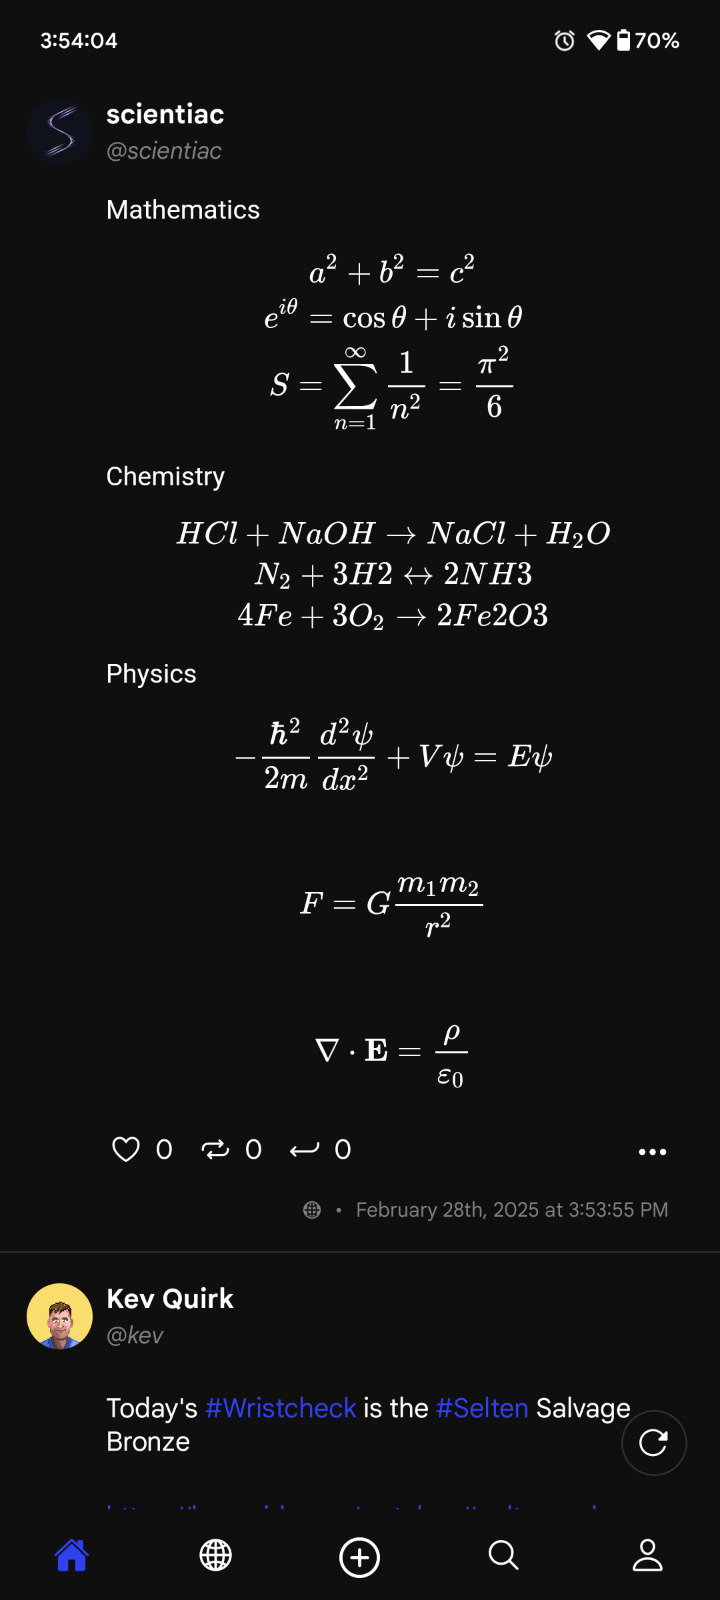
\includegraphics[width=\linewidth]{Graphics/postintimeline.png}
    \caption{Rendered post with latex in timeline}
  \end{minipage}
\end{figure}

\clearpage

\section{Interaction with Remote Accounts}


